\hspace{1.5cm}
Para uma distribuição e visualização da área de estudo é necessário realizar o recorte da mesma. Este processo é necessário para um bom trabalho, no processo digital de imagens. Isto faz com que o estudo se der somente na área de interesse do pesquisador. 

\begin{itemize}
\item \textbf{Basic Tools}
\begin{itemize}
\item \textbf{Layer Stacking} $\rightarrow$ \textbf{Spatial Subset}\\

\end{itemize}
\begin{figure}[!htpb]
        \centering
        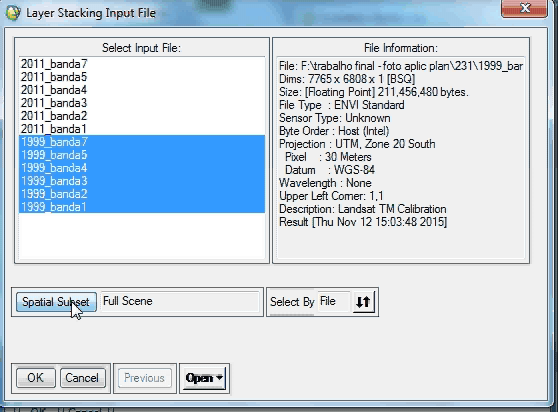
\includegraphics[scale =0.4]{imagens/corte04.png}
        \caption{Escolha dos Bandas para corte.}
        \label{corte04}
\end{figure}
\begin{figure}[!htpb]
        \centering
        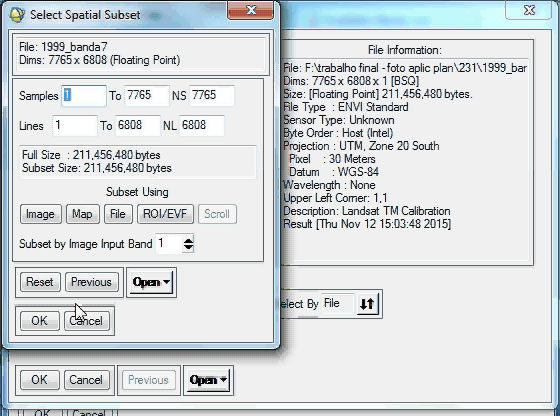
\includegraphics[scale=0.4]{imagens/corte05.png}
        \caption{Escolha dos Bandas para corte.}
        \label{corte05}
\end{figure}
\begin{figure}[!htpb]
        \centering
        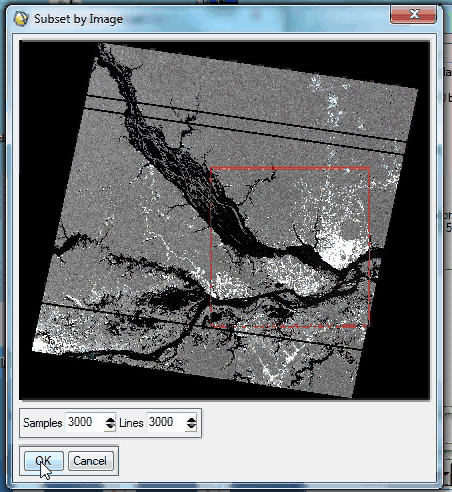
\includegraphics[scale=0.5]{imagens/corte06.png}
        \caption{Marcação da área para o corte.}
        \label{corte06}
\end{figure}
\end{itemize}
\hspace{1.5cm} Na figura \ref{corte04}, temos a escolha das bandas. A janela, figura \ref{corte05}, \textbf{Select Spatial Subset}, no primeiro momento escolhemos a opção \textbf{imagem} (figura \ref{corte06}). Já para realizá o a marcação das outras bandas utilizamos a opção \textbf{File} demonstra como foi feito o processo. O empilhamento é executado junto com o corte, na sequência.